\documentclass[a4paper,journal]{IEEEtran}
\usepackage{graphicx}
\usepackage{booktabs}
\usepackage{amsmath}
\usepackage{float}
\usepackage{verbatim}
%\usepackage{listings}
%\usepackage{array}
\usepackage{pdfpages}
\DeclareGraphicsExtensions{.pdf,.jpg}
\hyphenation{op-tical net-works semi-conduc-tor}

%\makeatletter
%\newcommand{\figcaption}{\def\@captype{figure}\caption}
%\newcommand{\tabcaption}{\def\@captype{table}\caption}
%\makeatother


\begin{document}
{\onecolumn \tableofcontents}
\thispagestyle{empty}


\twocolumn
\title{Congestion Control Mechanisms for Optical Burst Switched Networks}

\author{Fei Wang}

\markboth{MEng in Telecommunications Eng,August~2011}%
{Congestion Control Mechanisms for Optical Burst Switched Networks}

\maketitle



% Thesis Abstract -----------------------------------------------------


%\begin{abstractslong}    %uncommenting this line, gives a different abstract heading
\begin{abstracts}        %this creates the heading for the abstract page

    In this studies, I review burst congestion control problems in optical burst switching networks from the viewpoint of network throughput maximizaation and to reduce additional signal requirement while minimizing burst loss. Burst collision occurs when two or more bursts access the same wavelength at the same time, and the occurrence becomes more frequent with the offered load increases. 
    Burst must be dropped since OBS don't provide buffer on intermediate core router. That is said contention is inherent to the OBS network. There are a lot of predecessors have done a lot of research on this topic. General speaking, it has two jointly operating mechanisms, namely a burst congestion detection and a burst control algorithm. In this work, I want to overcome the shortcoming of previous research and develop a new mechanism to enhace OBS network stability and make
    congestion controllable. 
    \par
    {\bfseries Keyword:} Optical Switching Networks, Congestion Control

\end{abstracts}
%\end{abstractlongs}


% ----------------------------------------------------------------------


%%% Local Variables: 
%%% mode: latex
%%% TeX-master: "../thesis"
%%% End: 


\IEEEpeerreviewmaketitle


\section{Introduction}

\IEEEPARstart{O}{BS} has been proposed as strong candidate for the next generation
optical internet. OBS can achieve high statistical multiplexing and
provide flexible and dynamic bandwidth allocation required to support
highly dynamic and burst traffic\cite{ref:obs}.  In OBS networks, all input data
are assembled into a burst according to their destination in edge side, referred to
as data burstsd(DB), Shortly before the burst transmission begin, a
burst header cell(BHC) is sent on the control channel that is
processing on electric domain. The control packet BHC which contains 
information such as the destination address, the length of burst, the
number of hops it pass through and the burst offset time. BHC channel
is separated from the data burst channel. It take offset time to let 
the header cell be processed at each intermediate router before the data 
burst arrives. When all router along the path between source and destination 
complete resource reservation. DB can go through the path within whole
high-speed optical domain. The main different difference between an
optical network and a conventional packet switching network are
without optical buffer on the intermediate router. Once the network is congested,
some or all of bursts have to be dropped since bufferless on OBS. 
Hence, contention is inherent to the OBS technique and contention issue 
could affect tremendously the network performance in
terms of burst blocked rate and throughput. Recently, contention and loss
ratio may be reduced by implementing contention resolution policies,
such as time defection (using fiber delay line \cite{ref:fdl}), space 
deflection (using deflection routing \cite{ref:deflect}), and wavelength 
conversion \cite{ref:conversion}. These mechanisms can reduce burst blocked
rate in short-term burst congestion. But if the burst congestion 
lasts longer, the contention resolution policies can't handle any more. 
Some or all conflict bursts must be dropped. And then there are several soft contention
resolution policy can be applied for determining which bursts to drop.

The contention resolution policies are considered as reactive
approaches in the sense that they are invoked after contention occurs.
But also increase the complex implementation issues. An alternative
approach to avoid network contention and reduce burst loss is by proactively
 attempting to prevent network from overload through traffic management. This
paper focus on how to keep the rate of burst blocked rate of a network 
around a controllable level. An ideal congestion control mechanism should
achieve some objectives: enhance the throughput, reduce the average end-to-end burst delay, reduce data burst blocked rate, fair to all users and react timely. Basically, the congestion problem is due to the lack of information at the nodes and the absence of global coordination between the edge nodes and core nodes. As we know, in OBS, all intelligence resides in the edge nodes, which provides the buffer and the processor at the same time on the network. To solve these problems and consider about the feature of OBS, I develop a detect-feedback-react loop congestion control mechanism. 

The rest of the article is organized as follows.Section 2 stats the background of problem 
and related studies. The proposed congestion control scheme is illustrated in Section 3. 
Section 4 presents and analysis the computer experiment results. Finally, I concludes this paper in Section 5.


\section{Background, specification and related studies}

\subsection{Background and specification}

When there are too many bursts enter network, the performance of network will drop quickly. This phenomenon is known as congestion. 

\begin{figure}[!htb]
  \begin{minipage}[t]{0.5\linewidth} 
    \centering 
    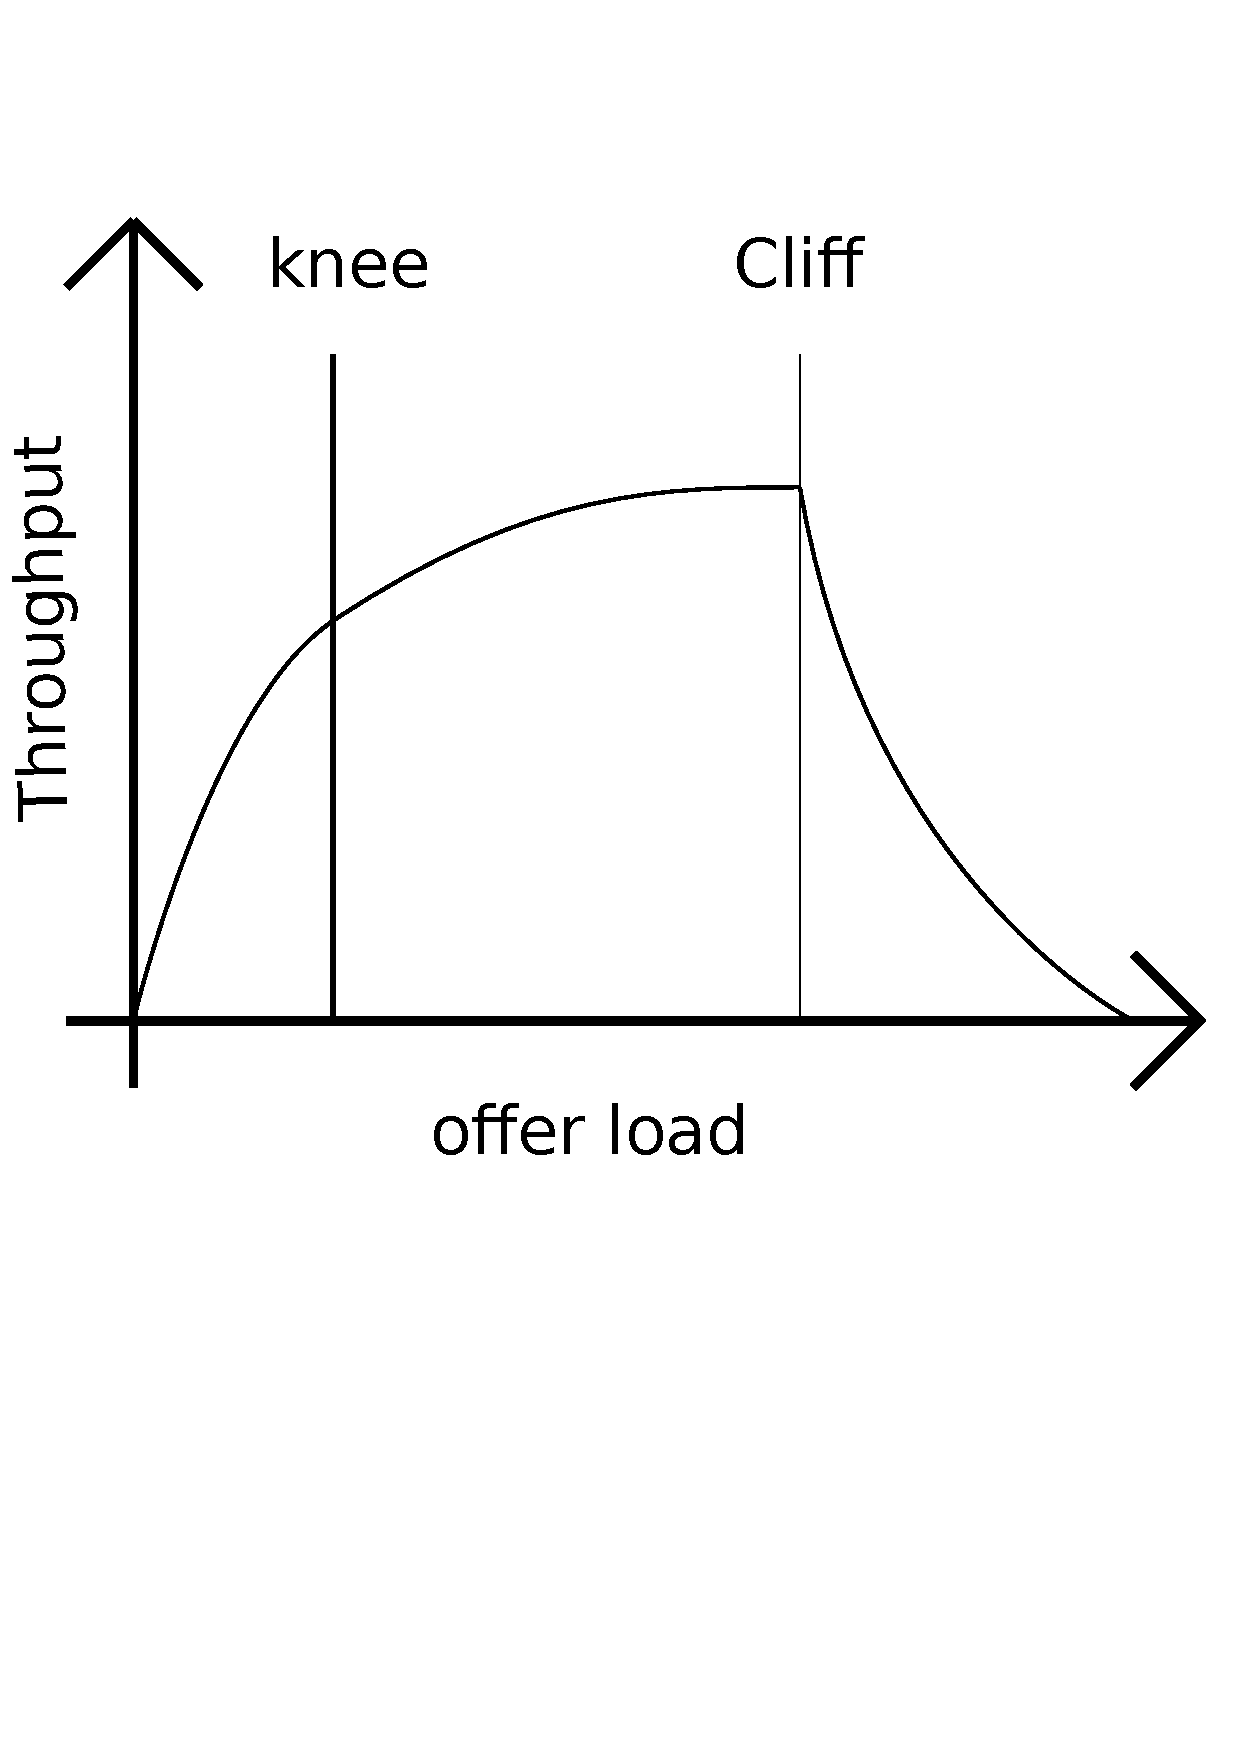
\includegraphics[width=1in]{fig/congestion_throughput} 
  \end{minipage}% 
  \begin{minipage}[t]{0.5\linewidth} 
    \centering  
    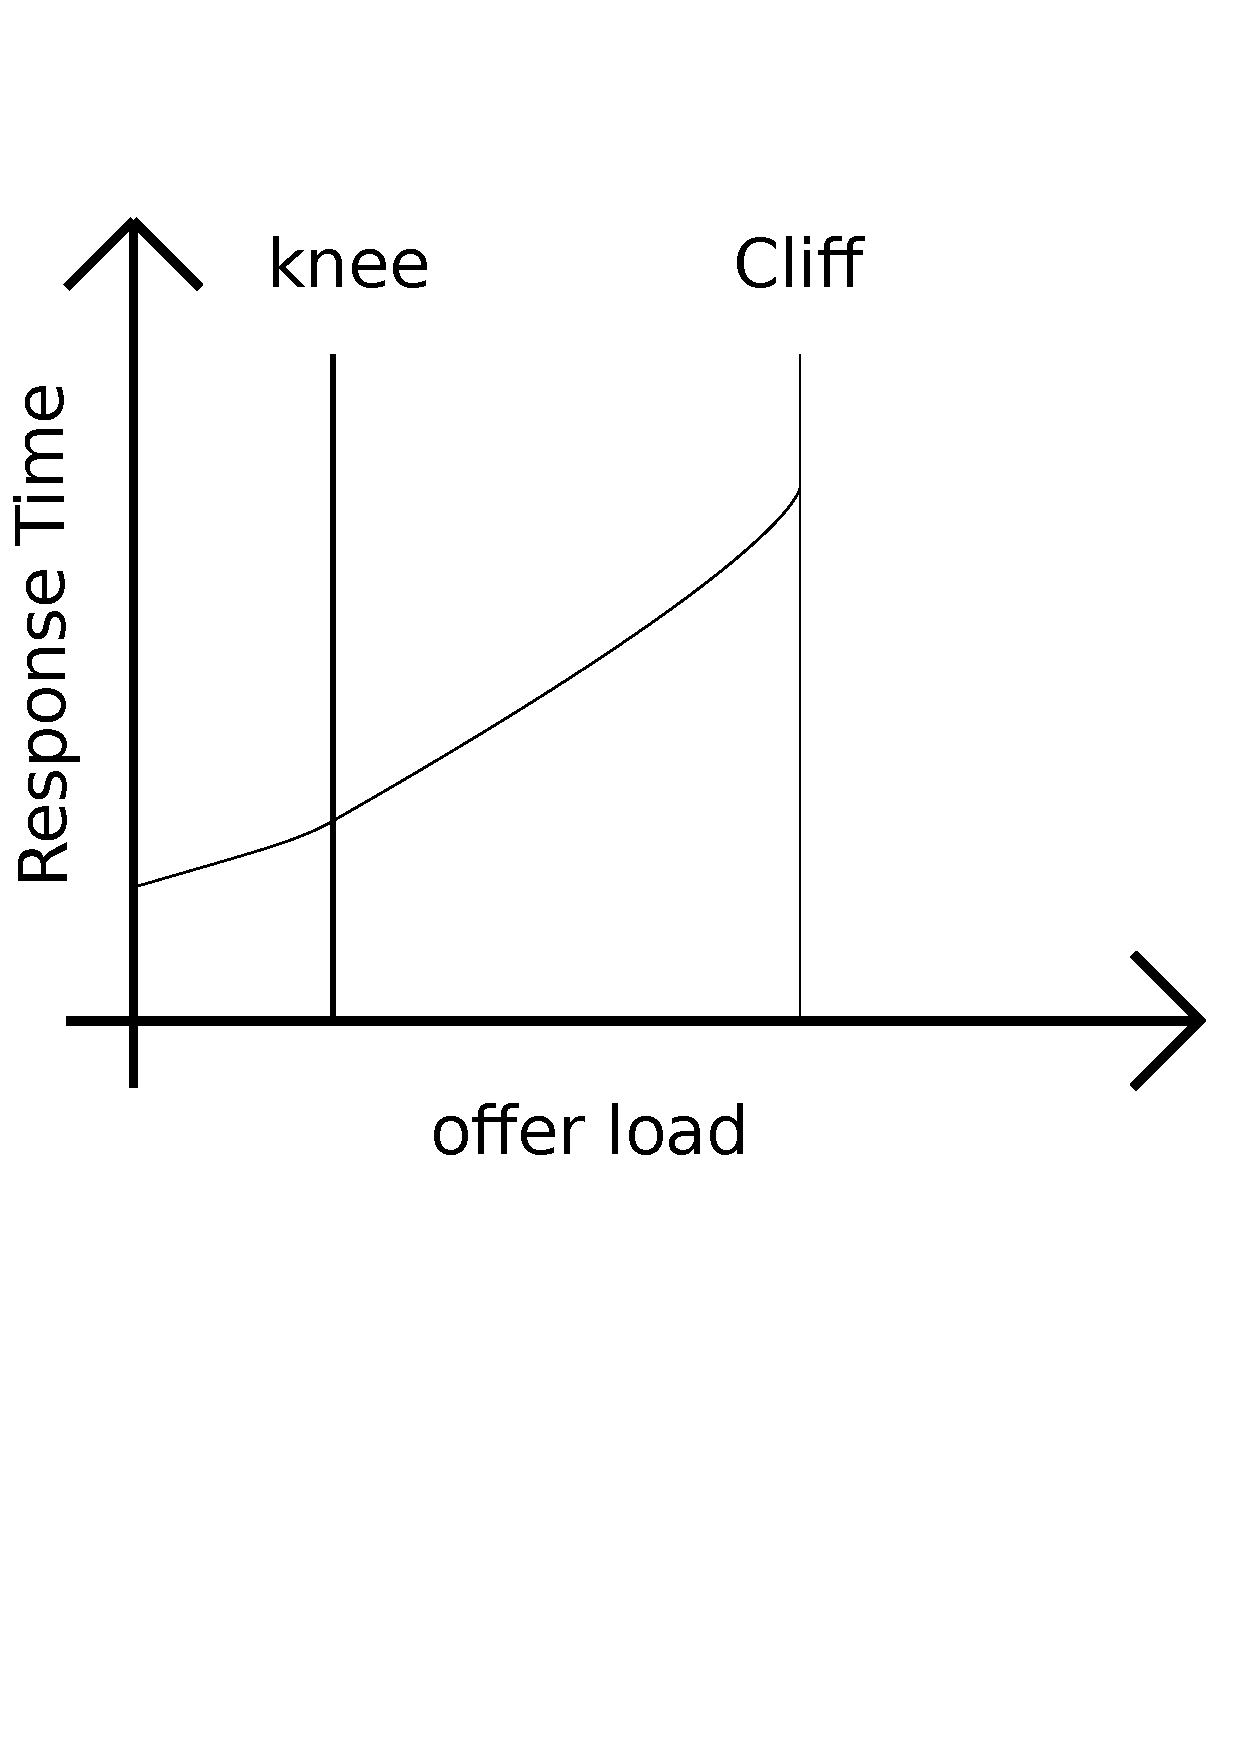
\includegraphics[width=1in]{fig/congestion_ete} 
  \end{minipage} 
  \caption{Congestive collapse}
  \label{fig:problem}
\end{figure}

As figure \ref{fig:problem} shown, when the offer load is low, the throughput of network increases linearly with offer load. The growth of response time is also slow. But when the offer load is higher than knee, the growth of throughput is slow but the response time increase sharply. When the offer load higher than cliff, the throughput fall sharply and response time shard rise. So the object of congestion control is to avoid network enter congestion and take action to clear out
congestion if it occurs. That is said keep the offer load stay between knee and cliff as long as possible.

\subsection{Related studies}

General speaking, there are two paradigms to handle congestion control. One with feedback message and the other without feedback message. For a non-feedback-based mechanism, also known as open-loop control, the edge routers have no information about the state of network and then cannot react to adjust the network offer load. All edge nodes regulate traffic load into network through traffic shaping or traffic rerouting and load balancing based on predefined traffic
description \cite{ref:feedback-based}. The challenge to implement the congestion control by non-feedback-based networks is to pre-determine the traffic parameter, such as average rate and distribution of arrival process at each edge. But also non-feedback-based control scheme can't adjust dynamically. The study of \cite{ref:peak-rate} is a typical open-loop mechanism. Recently, many researchers pay attention to feedback-based network, also refer as close-loop control. There are three stages in feedback-based control, that is detect,feedback,react. The paper \cite{ref:long-term-detect}
compare three detection algorithm. The first based on current traffic information, the second based on single statistic, the third based on multiple statistics. The author conclude that the multiple statistics help improving the estimation accuracy.  


\section{Feedback-based congestion control}

\subsection{Feedback control packet format}

\begin{figure}[!htb]
\centering
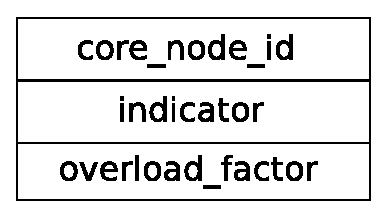
\includegraphics[width=2in]{fig/feedback_message}
\caption{Feedback Control Packet}
\label{fig:fcp}
\end{figure}

Figure \ref{fig:fcp} shows the feedback control packet fields.

core\_node\_id: indicate which core router send the feedback control packet.
Edge node can reroute to other available link according to this value.


indicator: the congestion status indicator. If congestion occurs, set to 1. Otherwise, set to 0.

overload\_factor: the percentage of burst blocked probability exceed the threshold. Edge node can determine the most congestion link with this value.

The feedback packets are broadcast to all associate ingress nodes periodically. In simulation, it is carried by a ICI format packet and assume without loss. On real network, they may transmitted within BHPs but with higher priority \cite{ref:real-network}. 

\subsection{Detection on core router}

Core routers are responsible for two main tasks: monitoring incoming bursts, broadcasting feedback control packet to the edge nodes.

The study of \cite{ref:long-term-detect} suggest multiple statistics improve estimation accuracy and react quickly. After balance the complexity and accuracy. I adopt the single statistic estimation algorithm. That is:

\begin{eqnarray*}
    B_{avg}(t) ~=~ (1-\alpha) \times B_{avg}(t-1) + \alpha \times B(t) \\
    0<\alpha<1
\end{eqnarray*}

Let $B_{avg}(t)$ denote the average data burst blocked probability of the samples at time $t$ with memory factor $\alpha$, where $B(t)$ is the current data burst blocked probability in a sample period $\tau$.

Then, the detection based on single statistic is,

\begin{enumerate}
\item if $B_{avg}(t) \geq B_{th}$, then congestion occurs 
\item otherwise, congestion clear out
\end{enumerate}

The implementation of this monitor can be found at \cite{ref:monitor}.

\subsection{Reaction on edge router}

The edge routers are responsible for receiving feedback congestion packet and adjust transmission rate inject into network through leaky bucket traffic shaping. As we know, each ingress router contains flow classifier, burst generation queue, leaky-bucket traffic shaper. Arriving BHPs move into corresponding burst queue according to their destination. 

Transmission rate are decided at the leaky bucket traffic shaper based on the feedback control packet at every core routers. For a given path, an optimal transmission rate is determined by the most-congested node on the path. 

$$
     R_{j,k}(i)=\left\{
                    \begin{aligned}
                     R_{j,k}(i-1) \times (1 + a) \quad B(i) \geq B_{th}\\
                     R_{j,k}(i-1) \times (1 - b) \quad B(i) < B_{th}
                    \end{aligned}
\right.
$$

Let $R_{i}$ denote the transmission rate of a certain path at the $i$th period. Where $a$ is the rate increasing factor and $b$ is the rate decreasing factor. Generally, $0<a<b<1$.  


The implementation of this leaky bucket rate controller can be found at \cite{ref:leaky-bucket}. 

\subsection{Determine parameter}

As the study of \cite{ref:feedback-based} suggest, the feedback mechanism and the parameter setup is very high relevant. So we need to determine the system parameter very carefully. In this part, I will explain how to determine the congestion threshold value and detect period.

Assume the inter-arrival time and service time of data burst meet the poisson distribution. Every fiber line contain $m$ available wavelength. The average arrival rate of DB is $\lambda$. The serve rate is $\mu$. Assume any input port DB scheduled to any wavelength of any output port. Thus, the output port can be considered as \verb|M/M/m/m| queueing system. Denote the traffic load $A=m\rho=m\frac{\lambda}{\mu}$. We can calculate the corresponding theory block probability according to
\verb|Erlang-B| formula. 

$$
    P_{block} ~=~ \frac{\frac{A^m}{m!}}{\sum_{i=0}^{m}\frac{A^i}{i!}}
$$

We can test this in single node value, When network load scale factor is 0.8, $\rho=1.2$, $m=10$, $P_{block} = 0.10$, when network load scale factor is 1.0, $\rho=1.5$, $P_{block} = 0.136$. We can find that is very closed to simulation result. As we know, if the congestion threshold value too low, it will impact the performance of network. On the opposite side, if this value is too high, the mechanism is restricted. So we can estimate the threshold value base this formula for
performance trade-off.  

Another important parameter is the period of detection and feedback. If this value low, the number of feedback control packets will increase and the performance of network will jitter sharply. If this time window last longer, the react of edge node will be slow. In this paper, I determine this value base on the end-to-end delay. That is 

$$ \tau = kT_{ete} $$

Where $T_{ete}$ is end-to-end delay. $\tau$ is the sampling period. For single node scenario, let $k=1000$. Through simulation result, I find that work well. How to determine this value is a complex problem, the study of \cite{ref:time-window} introduce a dynamic time windows congestion control.


\section{Simulation result}

This section present the simulation result based on the feedback-based congestion control. To simplify the problem. I start from a small network just contain single core router but with multiple edge routers. And then go through a normal network. The result demonstrated that congestion control police can reduce burst block ratio and prevent network from entering congestion status.

\begin{table}[!htb]
\renewcommand{\arraystretch}{1.3}
\caption{Common Parameter}
\label{tab:cp}
\centering
\begin{tabular}{l l}
\toprule
Parameter & Value \\
\midrule
Average Burst Length & 0.0001s \\
Number of Link Wavelengths & 10 \\
Use FDLs for Ingress Bursts     & no \\
Offset time & 0.0001s\\
Signaling and scheduling mechanisms & LAUC-AF \\
Weighted factor $\alpha$  & 0.5\\
Congestion detect period & 0.2 \\
Simulation Run Length & 5s \\
\bottomrule
\end{tabular}
\end{table}

Table \ref{tab:cp} show the common key parameters share with two scenarios. I also assume the inter-arrival time and burst service time of burst meet the exponential distribution. 

\subsection{Single node scenario}

\begin{figure}[!htb]
\centering
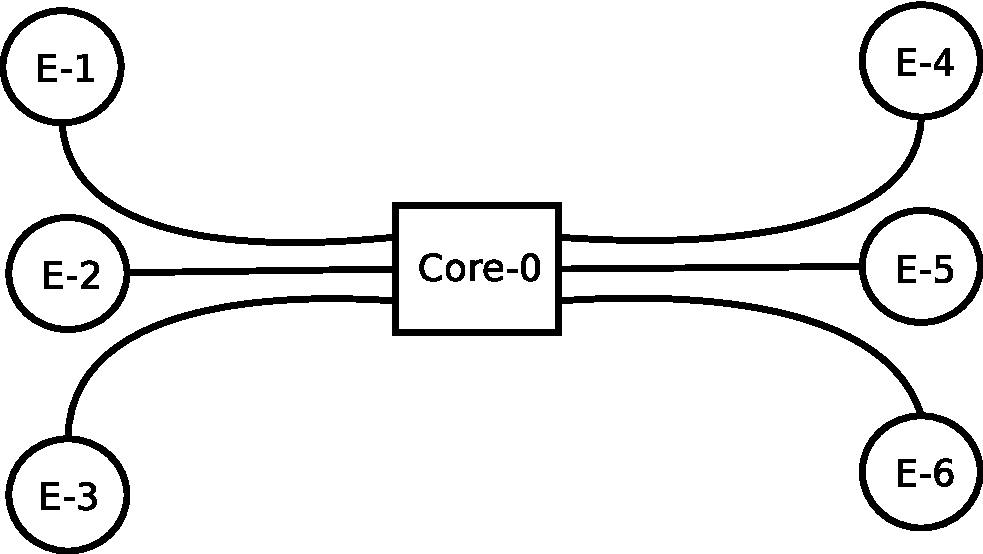
\includegraphics[width=2.6in]{fig/single_node_topo}
\caption{Single Node Network Model}
\label{fig:sn_topo}
\end{figure}

%\hspace{1pt}

Figure \ref{fig:sn_topo} shown the single node scenario topology and the routing table is shown below:

$$\begin{vmatrix}  
 1, & 4, & 1, & 0.5, & 1, & 0, & 4 \\  
 1, & 5, & 1, & 0.5, & 1, & 0, & 5 \\  
 1, & 6, & 1, & 0.5, & 1, & 0, & 6 \\  
 2, & 4, & 1, & 0.5, & 2, & 0, & 4 \\  
 2, & 5, & 1, & 0.5, & 2, & 0, & 5 \\  
 2, & 6, & 1, & 0.5, & 2, & 0, & 6 \\  
 3, & 4, & 1, & 0.5, & 3, & 0, & 4 \\  
 3, & 5, & 1, & 0.5, & 3, & 0, & 5 \\  
 3, & 6, & 1, & 0.5, & 3, & 0, & 6 \\  
\end{vmatrix}$$

The format of each row is:
\par
{\tt \{src, dest, svc\_level, load, path\}}

So there are nine paths. Every path pass through the single core node. For comparison purpose, I evaluate the performance of without congestion control mechanism and that employ feedback-based congestion control. Before us begin, we need to define some terms:

Network Load Scale: Specifies scaling factor for traffic offered to network. Each source generate rate calculate as (Network Load Scale) x (normalised load value) x (Link Wavelengths) / (Average Burst Length).

Burst block rate: average rate of data bursts that are blocked due to fail to schedule without available channel. 

Throughput: average rate of data bursts that are successfully transfer from source node to destination node.

\begin{figure}[!htb]
\centering
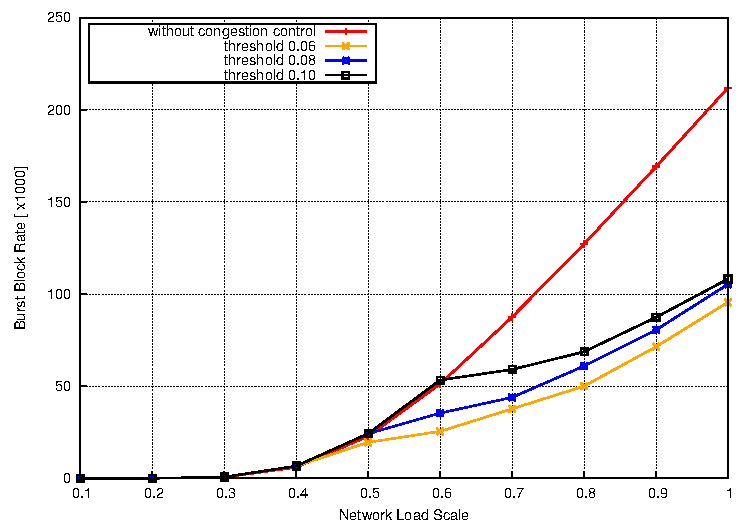
\includegraphics[width=2.6in]{result/single_node/block_rate_avg}
\caption{Burst Block Rate}
\label{fig:sn_block_rate}
\end{figure}

The burst block rate trend with the network load factor which start from 0.1 to 1.0 is show in the figure \ref{fig:sn_block_rate}. To the case without congestion control mechanism, the burst block rate keeps linearly increasing with the network load factor. When reach the bottleneck capacity of network, all arriving bursts will be blocked without any control. The performance would be reduced and network resource will be wasted. The case with congestion control and congestion threshold as 0.06
achieve the lowest burst blocked rate. Since the data burst inject into network will be limited at a lower rate. The figure shown the burst block rate also increases with network load factor. The ideal result will stay a certain value. This because of the simulation time is a little short. If it last longer, the shape of line would trend to be a horizontal line.

\begin{figure}[!htb]
\centering
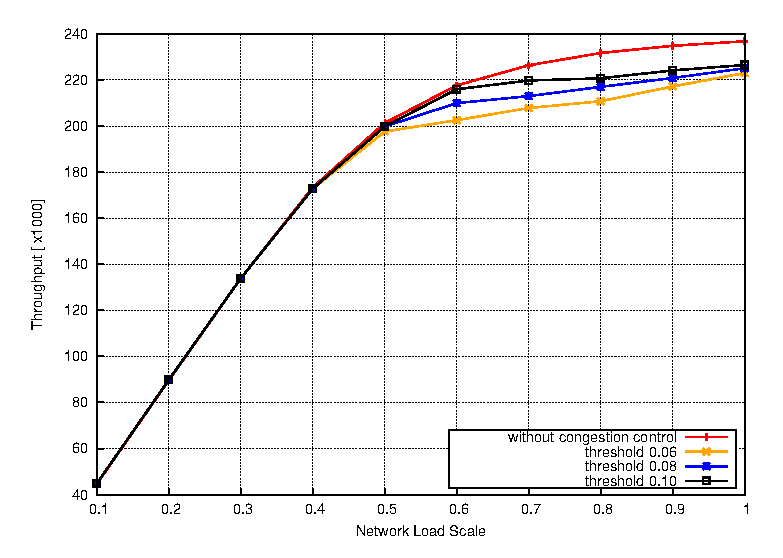
\includegraphics[width=2.6in]{result/single_node/throughput_avg}
\caption{Throughput}
\label{fig:sn_throughput}
\end{figure}

Figure \ref{fig:sn_throughput} compares the throughput of some case. As it illustrated, the throughput of case without congestion control gain the highest throughput. However, the growth of throughput is the expense of a highest burst block rate as shown in figure \ref{fig:sn_block_rate}. When network don't enter congestion, the throughput increase with the growth of network load scale. But if network is saturated, the throughput doesn't increase any more. The excess burst have to burst. This
figure also tell that the higher congestion threshold. Network can get higher throughput with higher blocking probability. Throughput and blocking probability trade-off should be consider.  

\begin{figure}[!htb]
\centering
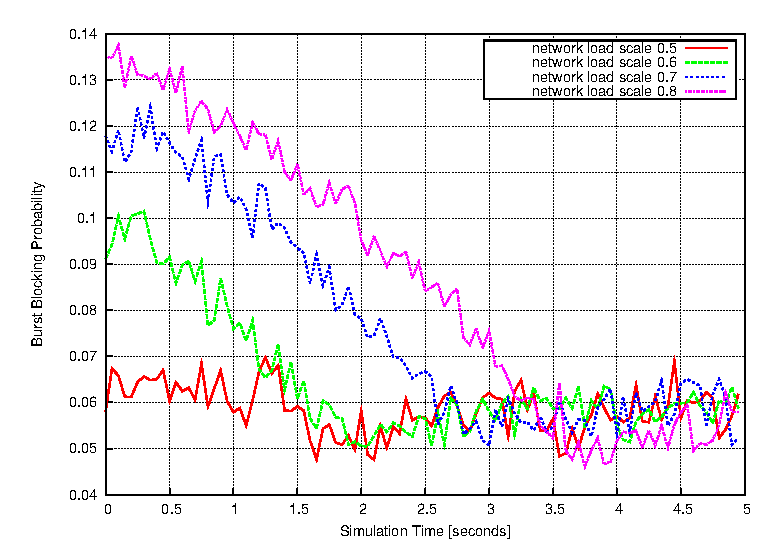
\includegraphics[width=2.6in]{result/single_node/block_probability_trend}
\caption{Block Probability Trend with Congestion Control}
\label{fig:sn_block_probability}
\end{figure}

Figure \ref{fig:sn_block_probability} shown the effect of feedback-based mechanism with congestion threshold 0.06. When network load scale factor is 0.5, the burst blocking probability jitter around the threshold with congestion control. With the growth of network load scale factor, the initial burst blocked probability increase sharply. That is said it will take longer to clear out the congestion status. But when it enter stable state, The feedback-based congestion control
scheme will limit the number of data burst inject to network and leaky bucket on edge side will smooth the traffic. The simulation result demonstrated that the mechanism can reduce the burst blocked probability even thought the network load scale increase high.

\subsection{Network scenario}

\begin{figure}[!htb]
\centering
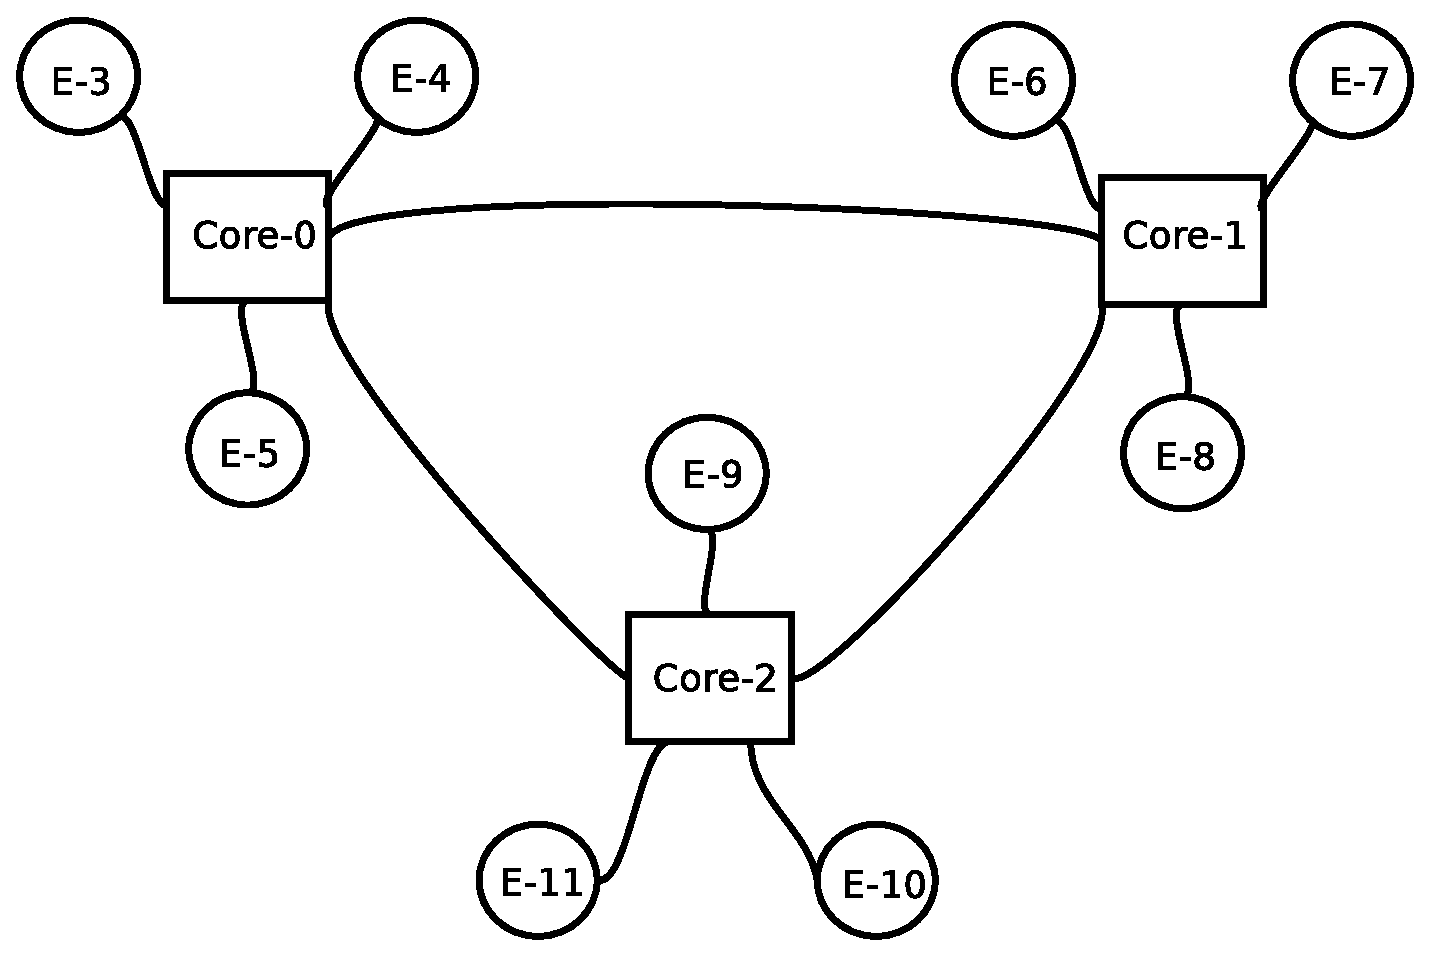
\includegraphics[width=2.6in]{fig/network_topo}
\caption{Network Model}
\label{fig:network_topo}
\end{figure}


Figure \ref{fig:network_topo} shown the network scenario topology and the routing table is shown below:

$$\begin{vmatrix}  
 3, & 6, & 1, & 0.5, & 3, & 0, & 1, & 6 \\  
 4, & 7, & 1, & 0.5, & 4, & 0, & 1, & 7 \\  
 5, & 8, & 1, & 0.5, & 5, & 0, & 1, & 8 \\  
 6, & 9, & 1, & 0.5, & 6, & 1, & 2, & 9 \\  
 7, & 10, & 1, & 0.5, & 7, & 1, & 2, & 10 \\  
 8, & 11, & 1, & 0.5, & 8, & 1, & 2, & 11 \\  
 9, & 3, & 1, & 0.5, & 9, & 2, & 0, & 3 \\  
 10, & 4, & 1, & 0.5, & 10, & 2, & 0, & 4 \\  
 11, & 5, & 1, & 0.5, & 11, & 2, & 0, & 5 \\  
\end{vmatrix}$$

There also are nine paths. However, every path pass through two core nodes. By analysing the routing table, these three core nodes are symmetrical to each others. So we just need to test if the mechanism works on any one of three core nodes. In this paper, I choose core node zero.

\begin{figure}[!htb]
\centering
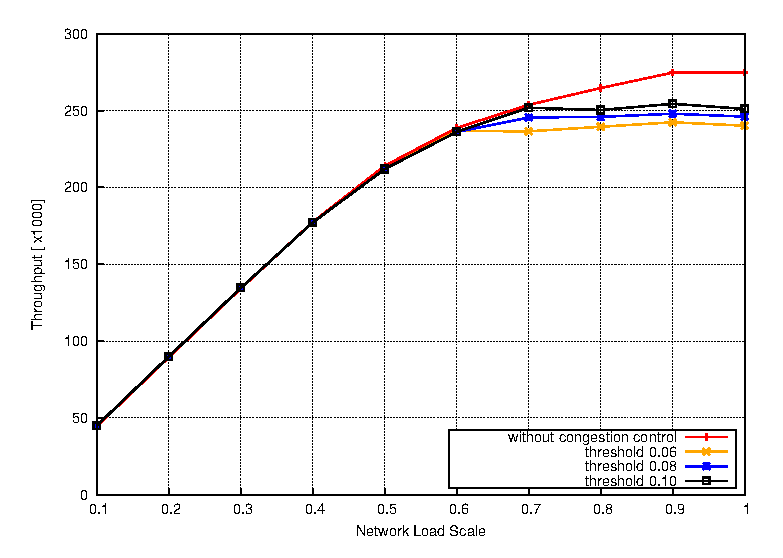
\includegraphics[width=2.6in]{result/network/throughput_avg}
\caption{Throughput}
\label{fig:net_throughput}
\end{figure}

As Figure \ref{fig:net_throughput} shown, the throughput of without any control is higher than with congestion control. The reason is similar to single node scenario.

\begin{figure}[!htb]
\centering
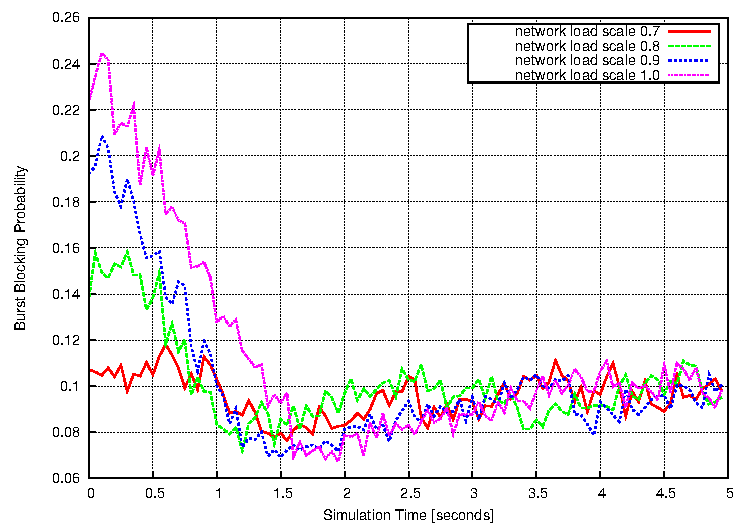
\includegraphics[width=2.6in]{result/network/block_probability_trend}
\caption{Block Probability Trend with Congestion Control}
\label{fig:net_block_probability}
\end{figure}

Figure \ref{fig:net_block_probability} shows the burst block probability of different network load scale factor during the simulation time with congestion threshold 0.1. It demonstrate that this mechanism can reduce the burst blocked probability in network environment. The cases with different network load scale factor almost achieve the threshold level at the same time. That is said the react delay doesn't increase with the arrival rate. 




\section{Conclusion}

In this paper, I proposed a congestion control mechanism based on feedback message sent from core router for OBS networks. Through the simulation result, I compared the overall data burst blocked rate for two cases, one with congestion control and the other without any control in single core node scenario and a small network scenario. It has been proven that this mechanism can reduce the burst blocked probability significantly. But also the throughput of network reduction, due to limit exceed data
burst inject to network, is tolerable. These and other topics, including implemented this mechanism with early dropping, behavior in larger network and what effect if core employ FDL line will focus on the future work.


% Can use something like this to put references on a page
% by themselves when using endfloat and the captionsoff option.
\ifCLASSOPTIONcaptionsoff
  \newpage
\fi

\bibliographystyle{IEEEtran}
\bibliography{reference}

\cleardoublepage
\setcounter{page}{2}
\renewcommand{\thepage}{\mbox{A-\arabic{page}}}

\addcontentsline{toc}{section}{Appendix}
\addcontentsline{toc}{subsection}{Appendix A -- A Survey of Congestion Control Mechanisms for Optical Burst Switched Networks}
\includepdfmerge{survey_cover.pdf,-}
\includepdfmerge{survey/survey.pdf,3-}

\cleardoublepage
\setcounter{page}{21}
\addcontentsline{toc}{subsection}{Appendix B -- Process model of leaky bucket}
\includepdfmerge{appendix/appendix_B.pdf,-}
\addcontentsline{toc}{subsection}{Appendix C -- Process model of monitor}
\includepdfmerge{appendix/appendix_C.pdf,-}


\end{document}


